\section{直接代数方法求$n$-孤子与1-lump的相互作用解}
\begin{frame}{求解非线性代数方程组的新算法}
随着非线性微分方程的应用领域不断拓宽, 从实际问题中产生的高维, 高阶甚至超维更复杂的非线性微分方程越来越多, 解的假设形式越来越复杂, 基于直接代数方法所获得的非线性代数方程组规模越来越大, 对于大规模非线性代数方程组的求解, 我们提出了以下两个算法: 

\begin{itemize}
\item 分组并行求解算法  
\item 继承求解算法  
\end{itemize}

为了得到大规模非线性代数方程组, 我们以求$n$-孤子与1-lump的相互作用解的直接代数方法为例进行说明. 
\end{frame}

\begin{frame}
\frametitle{直接代数方法求$n$-孤子与1-lump的相互作用解}
\begin{enumerate}
\item NS1L: 求$n$-孤子-1 lump相互作用解的软件包
\item PGSolve: 分组并行算法
\item 应用实例: (3+1)YTSF 方程
\item 求解效率对比
\item 软件展示 
\end{enumerate}
\end{frame}

\subsection{NS1L: 求n孤子-1 lump相互作用解的软件包}
\begin{frame}{NS1L: 求n孤子-1 lump相互作用解的软件包}
考虑非线性演化方程
\[
    U(u,u\up{1},u\up{2},\cdots)=0 
\]
其中 $u=u(x_1,\cdots,x_m)$. 假设原方程存在 Painleve 截断展开  
\[
    u=\sum_{k=1}^m{\frac{u_k}{f^{m-k+1}}}
\]
基于$n$阶展开方法, 我们可以确定$m$的上界, 从而确定这个变换的具体表达式. 将上述变换代入原方程, 可以得到关于$f$及其导数的方程
\[
    F(f,f\up{1},f\up{2},f\up{3}\cdots)=0
\]
\end{frame}
\begin{frame}
\small 
用直接代数方法求$n$-孤子和1-lump的相互作用解时, 我们假设$f$具有如下形式 
\[
    f_n=\sbrace{\xi_1+\eta_1}^2+\sbrace{\xi_2+\eta_2}^2+\sum_{i=1}^{2^n}\sbrace {q_i\prod_{k \in T_i}{\exp(\xi_{k+2})}}
\]
\[
    \xi_k=\sum_{j=1}^m{p_{j,k}x_j}=p_{1,k}x_1+\cdots+p_{m,k}x_m
\]
$T_i$是$\bbrace{1,2,\cdots,n}$的第$i$个子集. 子集顺序为
\[
    \emptyset,\bbrace{1},\bbrace{2},\bbrace{1,2},\bbrace{3},\bbrace{1,3},\bbrace{2,3},\bbrace{1,2,3},\cdots 
\]
从而, 高阶解能够退化为相同形式的低阶解, 这是能够继承求解的前提条件. 例如, 
\[
\begin{aligned}
    f_1 &= \sbrace{\xi_1+\eta_1}^2+\sbrace{\xi_2+\eta_2}^2+q_1+q_2 \exp(\xi_3) \\ 
    f_2 &= \sbrace{\xi_1+\eta_1}^2+\sbrace{\xi_2+\eta_2}^2+q_1+q_2 \exp(\xi_3) \\
        & +q_3 \exp(\xi_4) + q_4 \exp(\xi_3+\xi_4)
\end{aligned}
\]
\end{frame}

\begin{frame}
约束条件:
\begin{itemize}
\item 孤子解的各个相互作用系数非零.
\item 行波中各个变量的系数不能全为零. 
\item lump 解部分不退化.
\item 孤子解部分不退化. 
\end{itemize}
相应的避免取值集合为: 
\[
\begin{aligned}
    S&=\bbrace{\bbrace{q_i=0}|2\le i \le 2^n} \\ 
        &\cup \bbrace{\bbrace{p_{1,k}=0,\cdots,p_{m,k}=0}|1\le k \le n+2}  \\
        &\cup \bbrace{\bbrace{p_{j,1}=0,p_{j,2}=0}|1\le j \le m} \\ 
        &\cup \bbrace{\bbrace{p_{j,3}=0,\cdots,p_{j,n+2}=0}|1\le j \le m} .  
\end{aligned}
\]
对于一个解$sol$ (是一个集合), 若存在$s\in S$, 满足$s\subseteq sol$, 则$sol$就不是我们想要的解.
\end{frame}

\subsection{PGSolve: 分组并行求解算法}
\begin{frame}
\frametitle{PGSolve: 分组并行求解算法}
\begin{figure}
\centering
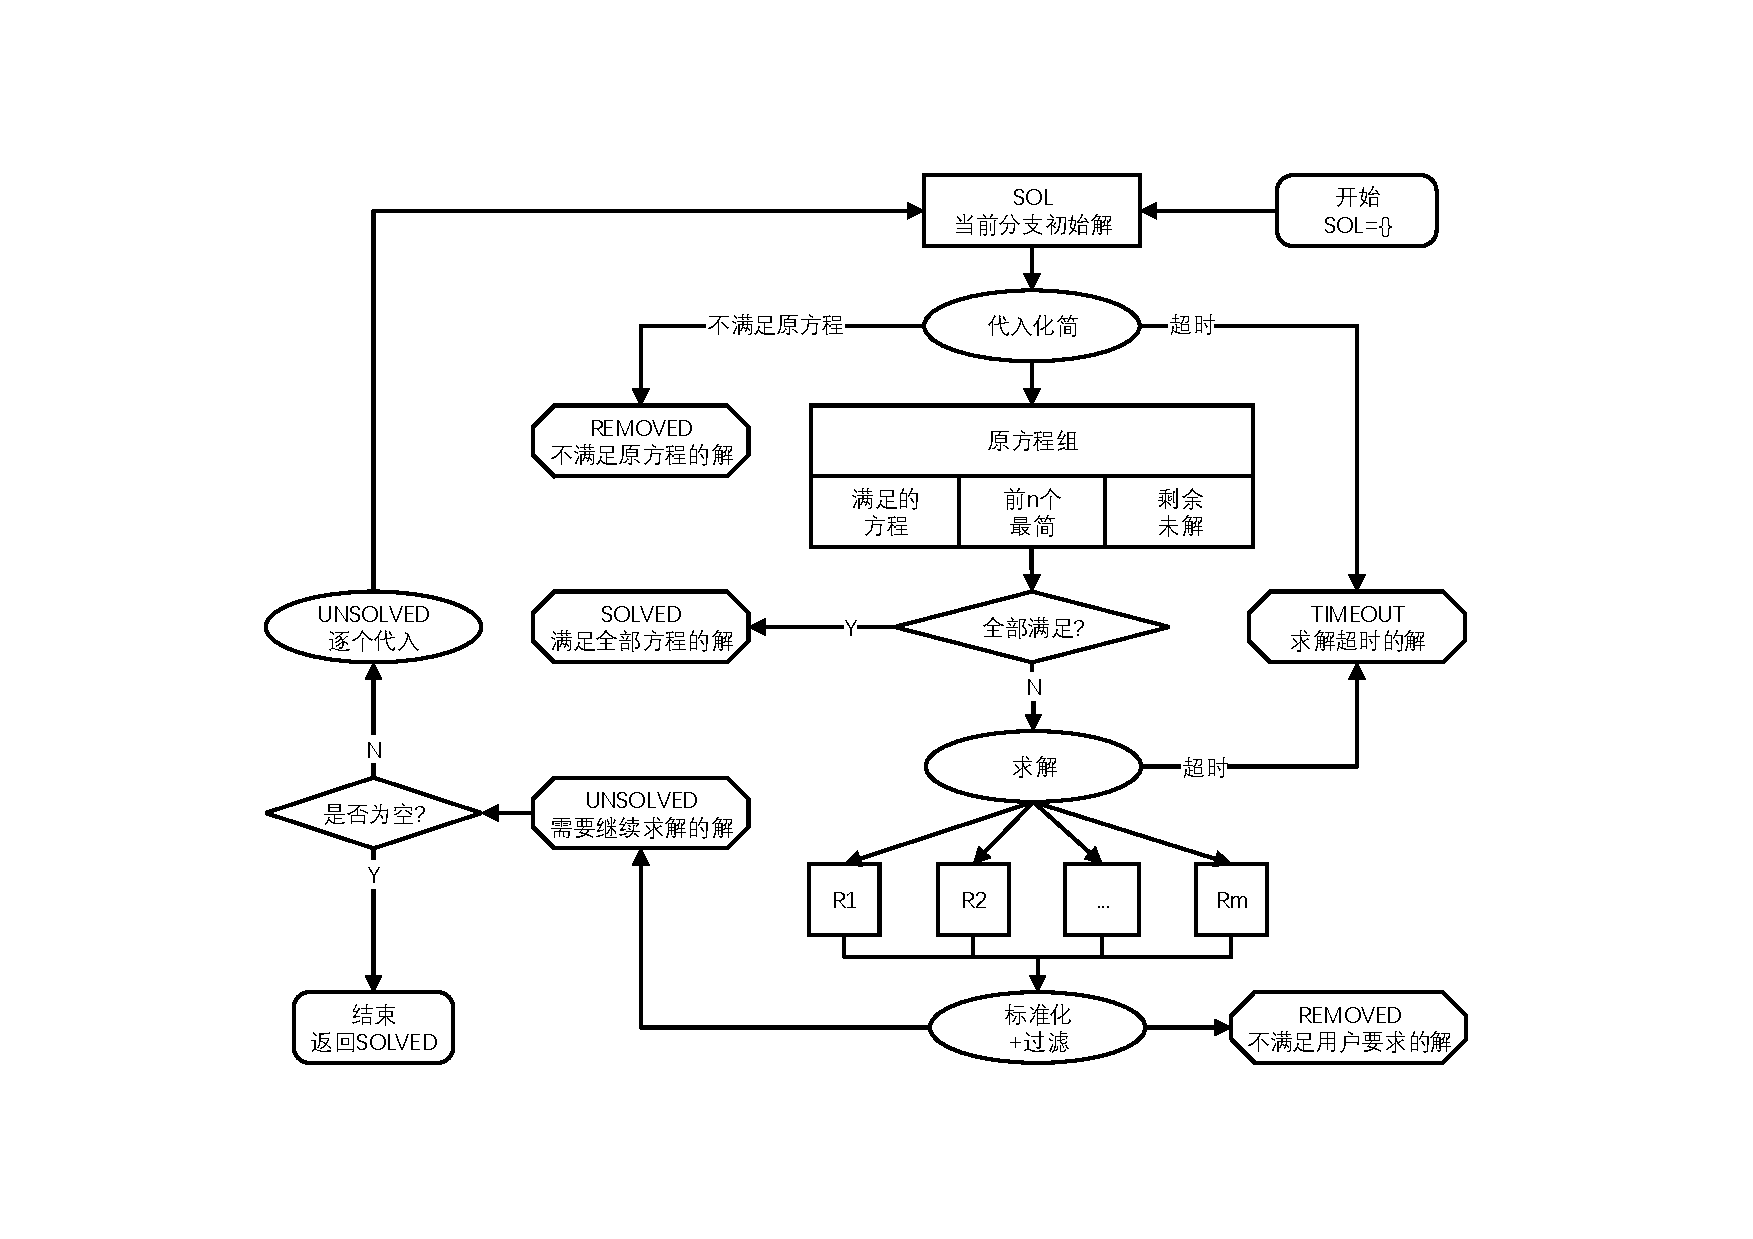
\includegraphics[height=0.8\textheight]{../paper/fig/pgsolve.pdf}
\end{figure}
\end{frame}

\begin{frame}
代入化简所有方程的优势:
\begin{enumerate}
\item 对尚未求解的方程进行代入化简, 能够对新的方程组按照复杂度重新排序, 从而获得更简单的方程.
\item 对已经求解过的方程进行代入化简, 能够验证当前分支的解是否满足这部分方程. 
\item 虽然单个分组只求解了$n$个方程, 但是获得的解可能满足更多的方程, 代入后可以及时地减少待求解方程的数量. 
\end{enumerate}
\end{frame}

\subsection{应用实例: (3+1)YTSF 方程}
\begin{frame}{应用实例: (3+1)YTSF 方程}
\[
    3\,\alpha\,u_{{{\it yy}}}+4\,u_{{x}}u_{{{\it xz}}}+2\,u_{{{\it xx}}}u_{{z}}-4\,u_{{{\it tx}}}+u_{{{\it xxxz}}}=0. 
\]
在接下来的例子中, 分组大小 $n=5$. 

\[
\begin{aligned}
    f_0 &=\sbrace{\xi_1+\eta_1}^2+\sbrace{\xi_2+\eta_2}^2 \\ 
    f_1 &= \sbrace{\xi_1+\eta_1}^2+\sbrace{\xi_2+\eta_2}^2+q_1+q_2 \exp(\xi_3) \\ 
    f_2 &= \sbrace{\xi_1+\eta_1}^2+\sbrace{\xi_2+\eta_2}^2+q_1+q_2 \exp(\xi_3) \\
        & +q_3 \exp(\xi_4) + q_4 \exp(\xi_3+\xi_4)
\end{aligned}
\]
\end{frame}
\begin{frame}
\begin{figure}
\centering
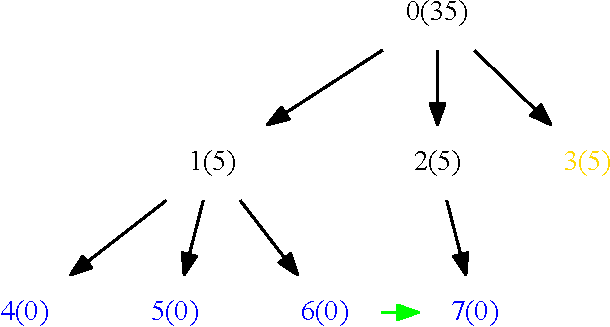
\includegraphics[width=.5\textwidth]{../paper/fig/0S1L.pdf}
\caption{0S-1L 求解分支图 (1秒)}
\end{figure}
\end{frame}

\begin{frame}
\begin{figure}
\centering
\setcounter{subfigure}{0}
\subfigure[]{
    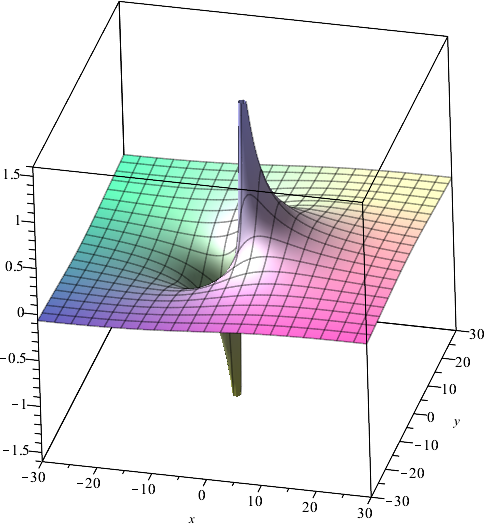
\includegraphics[width=.3\textwidth]{../paper/fig/0S1L-1.png}
}
\subfigure[]{
    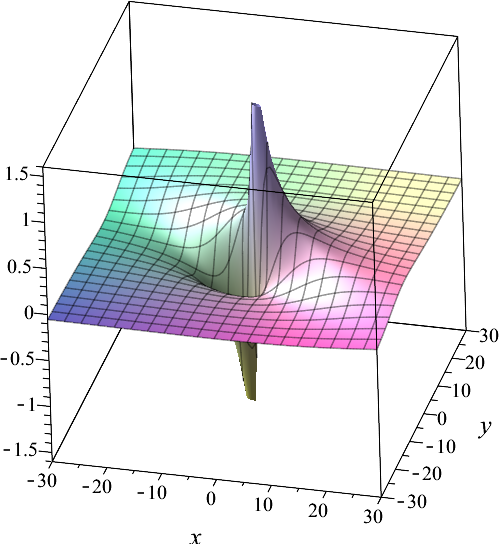
\includegraphics[width=.3\textwidth]{../paper/fig/0S1L-2.png}
}
\caption{(3+1)维 YTSF 方程的 0S-1L 解}
\end{figure}
\end{frame}


\begin{frame}
\begin{figure}
\centering
\setcounter{subfigure}{0}
\subfigure[1S-1L直接求解(8秒)]{
    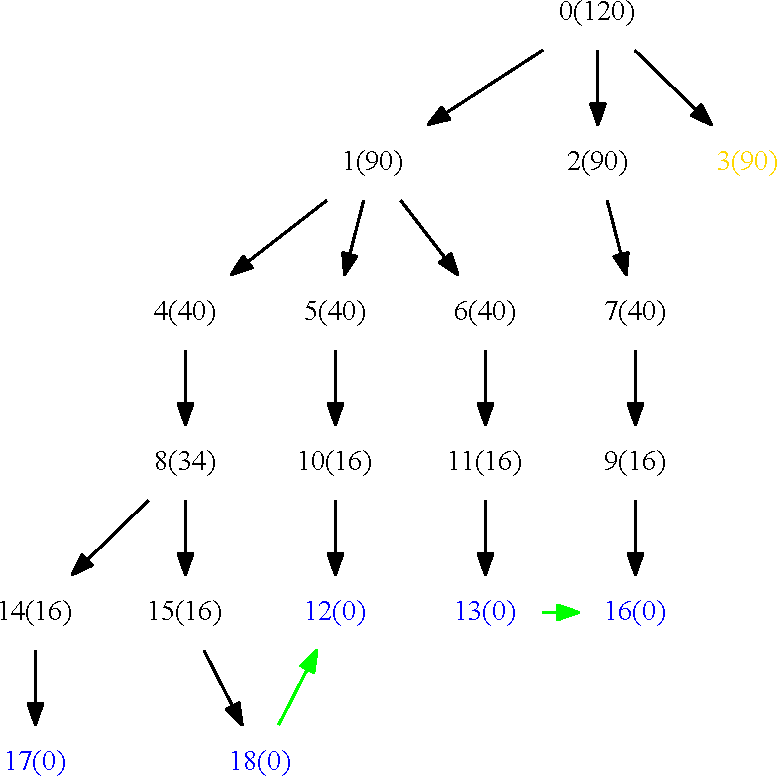
\includegraphics[width=.4\textwidth]{../paper/fig/1S1L-dir.pdf}
}
\hspace{2cm}
\subfigure[1S-1L继承求解(5秒)]{
    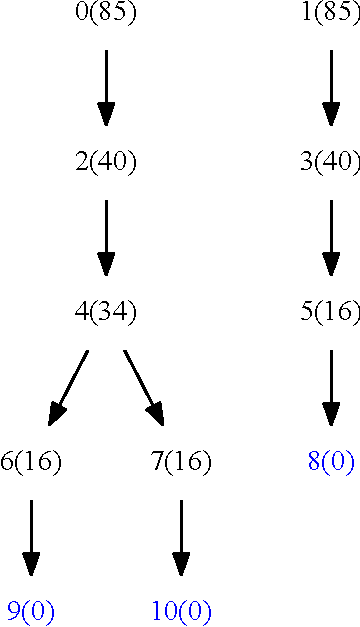
\includegraphics[width=.28\textwidth]{../paper/fig/1S1L-ext.pdf}
}
\end{figure}
\end{frame}

\begin{frame}
\begin{figure}
\centering
\setcounter{subfigure}{0}
\subfigure[]{
    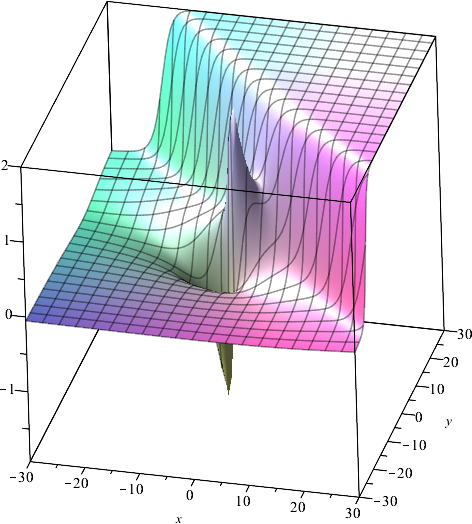
\includegraphics[width=.3\textwidth]{../paper/fig/1S1L-1.png}
}
\subfigure[]{
    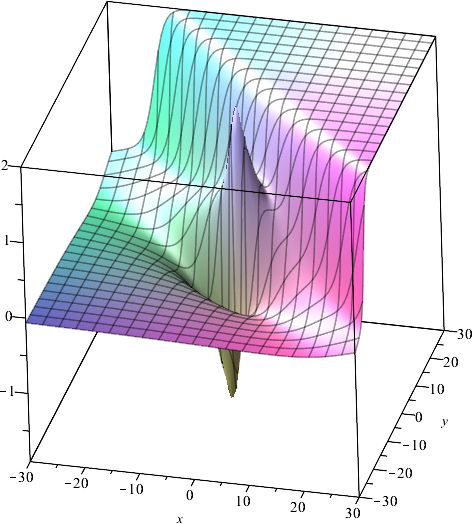
\includegraphics[width=.3\textwidth]{../paper/fig/1S1L-2.png}
}
\subfigure[]{
    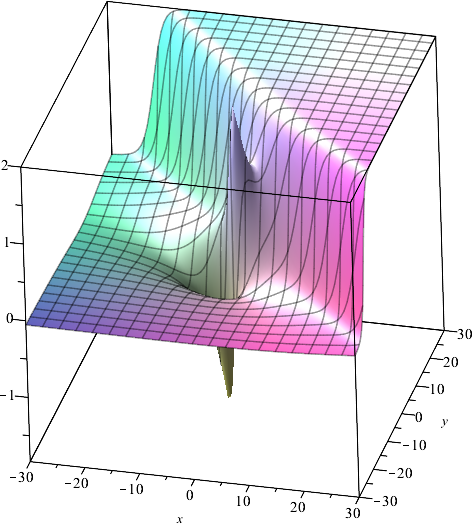
\includegraphics[width=.3\textwidth]{../paper/fig/1S1L-3.png}
}
\caption{(3+1)维 YTSF 方程的 1S-1L 解} \label{fig-1S1L}
\end{figure}
\end{frame}

\frame{
\begin{figure}
\centering
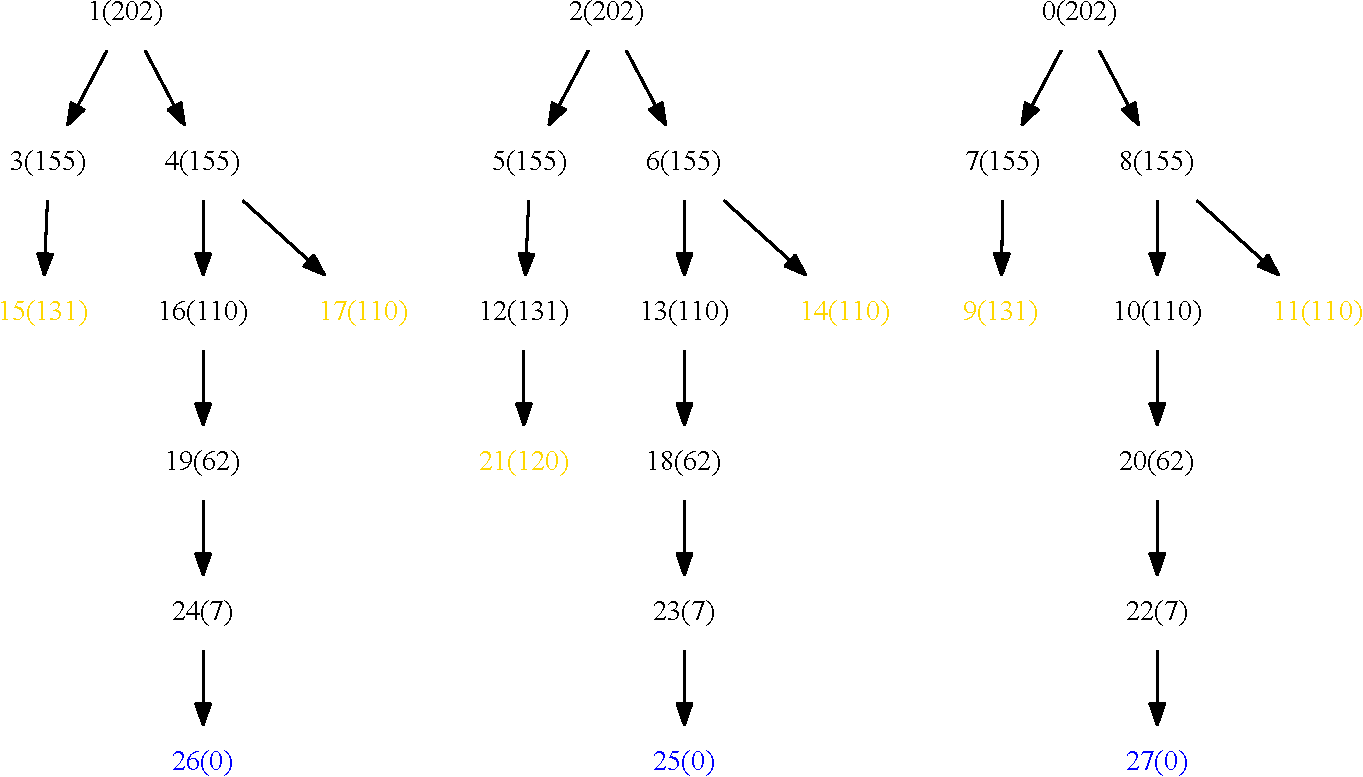
\includegraphics[width=\textwidth]{../paper/fig/2S1L-ext.pdf}
\caption{2S-1L 继承求解的分支图(30 秒)}\label{sb2-e}
\end{figure}
}

\begin{frame}
\begin{figure}
\centering
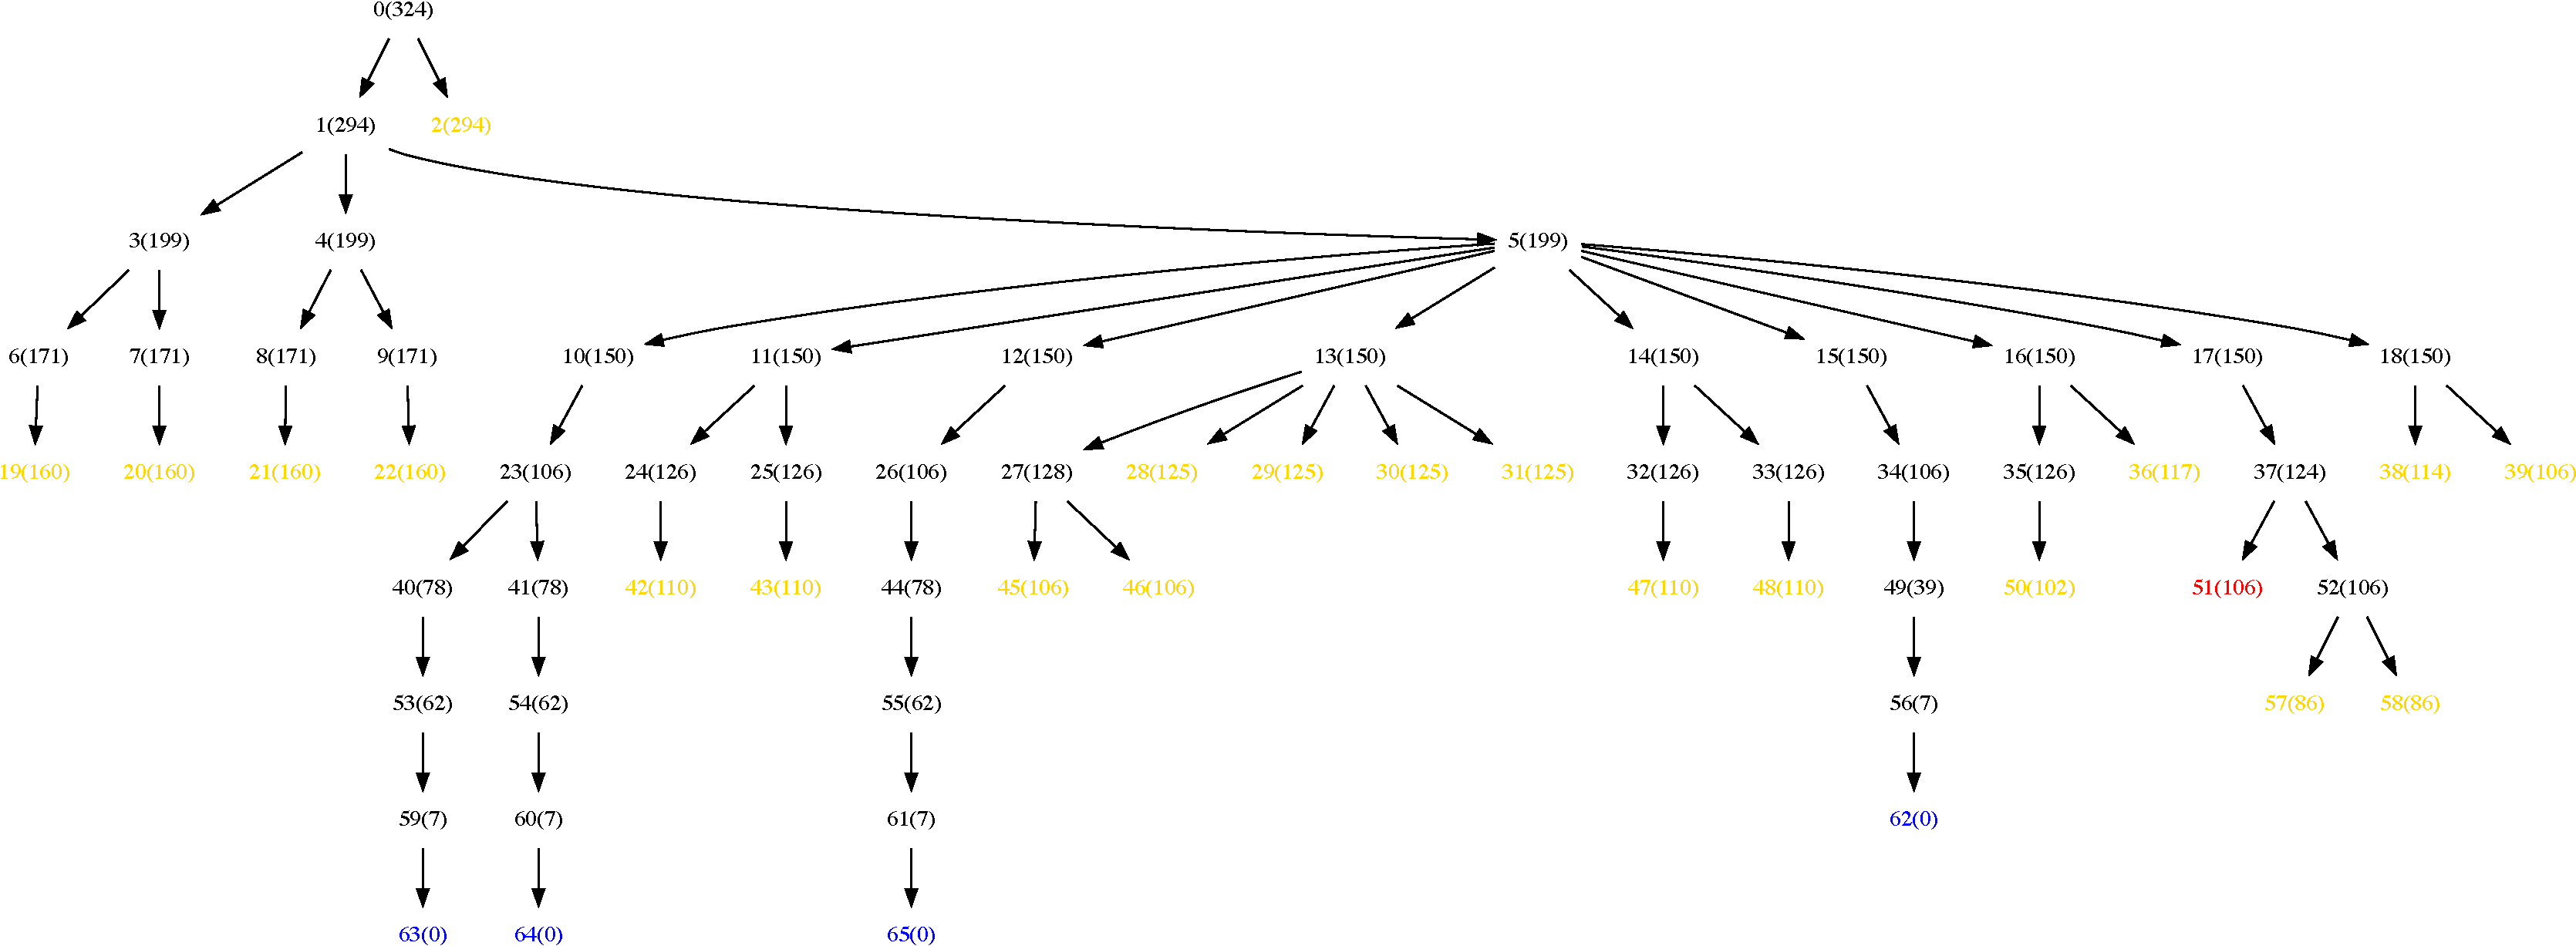
\includegraphics[width=\textwidth]{2S1L-dir-number.pdf}
\caption{2S-1L 直接求解的分支图(430 秒)}\label{sb2-d-n}
\end{figure}
\end{frame}

\frame{
\begin{figure}
\centering
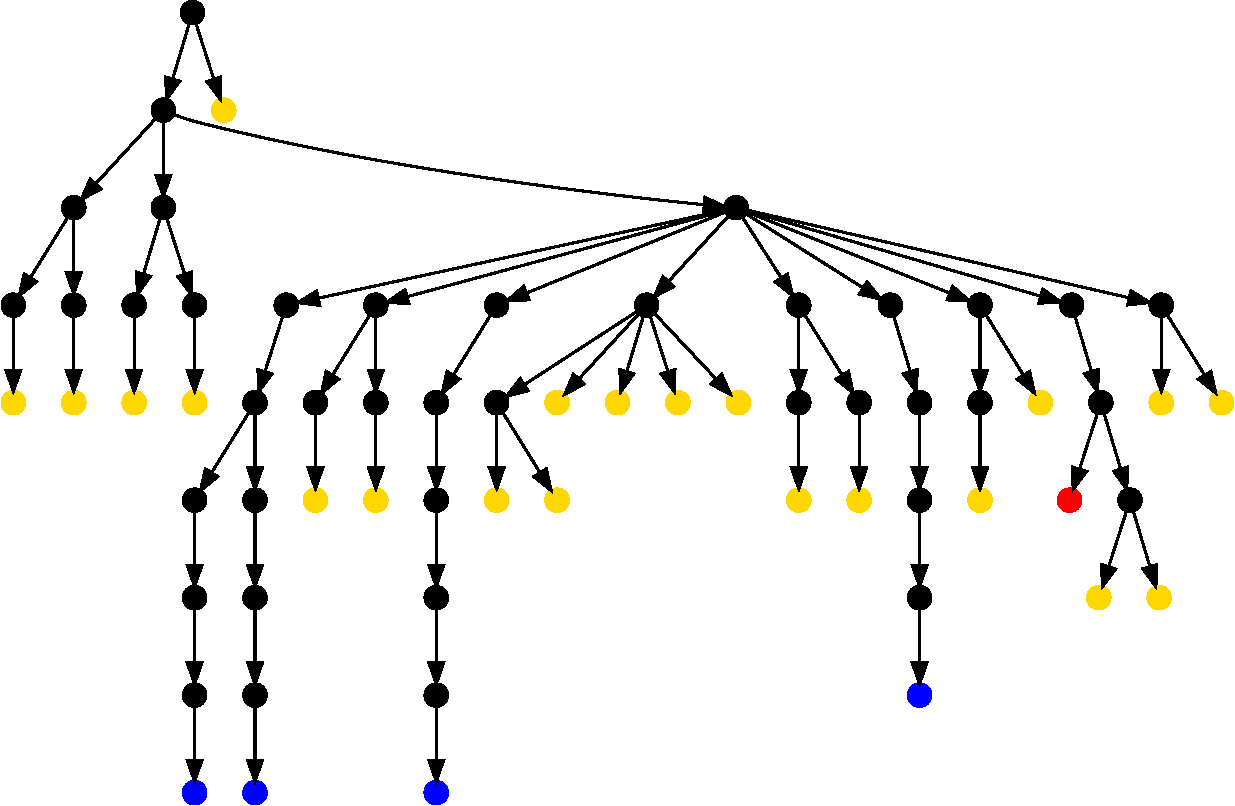
\includegraphics[height=0.8\textheight]{2S1L-dir-point.pdf}
\caption{2S-1L 直接求解的分支图(430 秒)}\label{sb2-d-p}
\end{figure}
}

\frame{
\begin{figure}
\centering
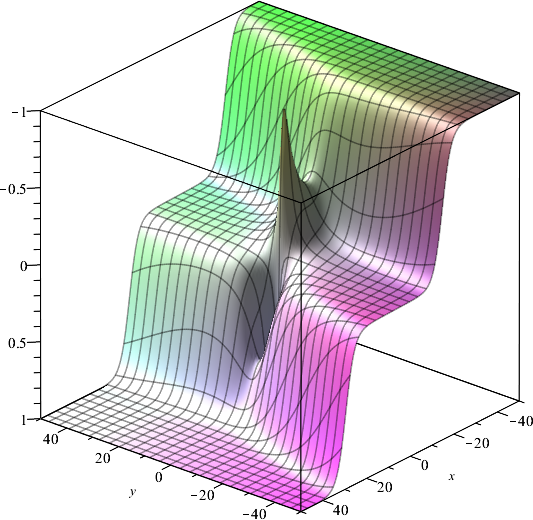
\includegraphics[width=.6\textwidth]{../paper/fig/2S1L.png}
\caption{(3+1)维 YTSF 方程的 2S-1L 解} \label{fig-2S1L}
\end{figure}
}

\subsection{求解效率对比}
\begin{frame}
\frametitle{求解效率对比}
\begin{adjustbox}{max width=\textwidth}
\centering
\renewcommand{\arraystretch}{1.3}
\begin{tabular}{cccccc}
\hline
来源方程 & 阶数 & 方程数 & 变量数 & PGSolve用时 & Solve用时 \\
\hline
(2+1) SK & 0 & 20 & 9 & 0.724 & 3.483 \\
(2+1) BKP-T & 0 & 20 & 9 & 0.571 & 3.486 \\
(2+1) KP & 0 & 35 & 9 & 1.759 & 29.643 \\
(3+1) YTSF & 0 & 35 & 11 & 1.229 & 8.839 \\
(3+1) JM & 0 & 35 & 11 & 0.845 & >1800 \\
(2+1) SK & 1 & 65 & 13 & 10.241 & >1800 \\
(3+1) YTSF & 1 & 120 & 16 & 12.228 & 1696.852 \\
\hline
\end{tabular}
\end{adjustbox}

\vspace{1em}

此处对比的是\cd{PDEtools:-Solve}. 而最常用的\cd{solve}函数甚至不能在 72 小时内求解只有 20 个方程的方程组, 这显然是\cd{solve}函数的一个 BUG.

\end{frame}

\begin{frame}

\begin{adjustbox}{max width=\textwidth}
\renewcommand{\arraystretch}{1.3}
\begin{tabular}{cccccc}
\hline
方程名称    & 解的阶数 & 方程数量 & 分组大小 & 解的个数 & 运行时间(s) \\ 
\hline 
(2+1)SK & 0 & 20 & 5 & 1 & 2.197 \\
(2+1)SK & 1 & 65 & 3 & 1 & 3.072 \\
(2+1)SK & 2 & 179 & 5 & 2 & 12.697 \\
(2+1)BKP-T & 0 & 20 & 5 & 1 & 1.036 \\
(2+1)BKP-T & 1 & 65 & 3 & 1 & 3.251 \\
(2+1)BKP-T & 2 & 179 & 5 & 2 & 12.617 \\
(3+1)YTSF & 0 & 35 & 5 & 2 & 1.948 \\
(3+1)YTSF & 1 & 120 & 5 & 3 & 6.717 \\
(3+1)YTSF & 2 & 324 & 5 & 3 & 37.909 \\
(3+1)JM & 0 & 35 & 5 & 3 & 2.014 \\
(3+1)JM & 1 & 120 & 5 & 13 & 18.384 \\
(3+1)JM & 2 & 324 & 5 & 4 & 50.934 \\
\hline 
\end{tabular}
\end{adjustbox}

\end{frame}

\subsection{软件展示}
\begin{frame}{软件展示}
\href{run:../LypReportProgram/NS1L.mw}{NS1L.mw}
\begin{itemize}
\item 0S-1L 直接求解 
\item 1S-1L 直接求解和继承求解的对比
\item 2S-1L 继承求解
\end{itemize}
\end{frame}